\section{System Overview}
\label{sec:system}

\subsection{Design principle: the candidate is the unit of research}

\system treats a materials campaign as the evolution of a set of scientific objects rather than the generation of a sequence of answers.  The central object is a \emph{candidate record}.  It binds a stable material identity to five kinds of state: the constraints against which the candidate is judged, the evidence supporting those judgements, the parent or generated crystal structure, the computations scheduled for that structure, and the decisions that determine its subsequent trajectory.  A candidate may begin as a database structure, a literature mechanism, or a model-proposed composition.  In each case, the same record is enriched rather than replaced as the campaign progresses.

This representation is useful because materials questions are usually underdetermined at the moment they are posed.  A database may establish that a structure is two-dimensional but contain no evidence about the orbital character of a band; a paper may motivate a mechanism without providing a machine-readable structure; and a generated child may be geometrically valid before its electronic state is known.  The system therefore permits incomplete candidate records while requiring every populated field to retain its source.  Missing observations remain explicit targets for subsequent work.

\begin{figure}[t]
    \centering
    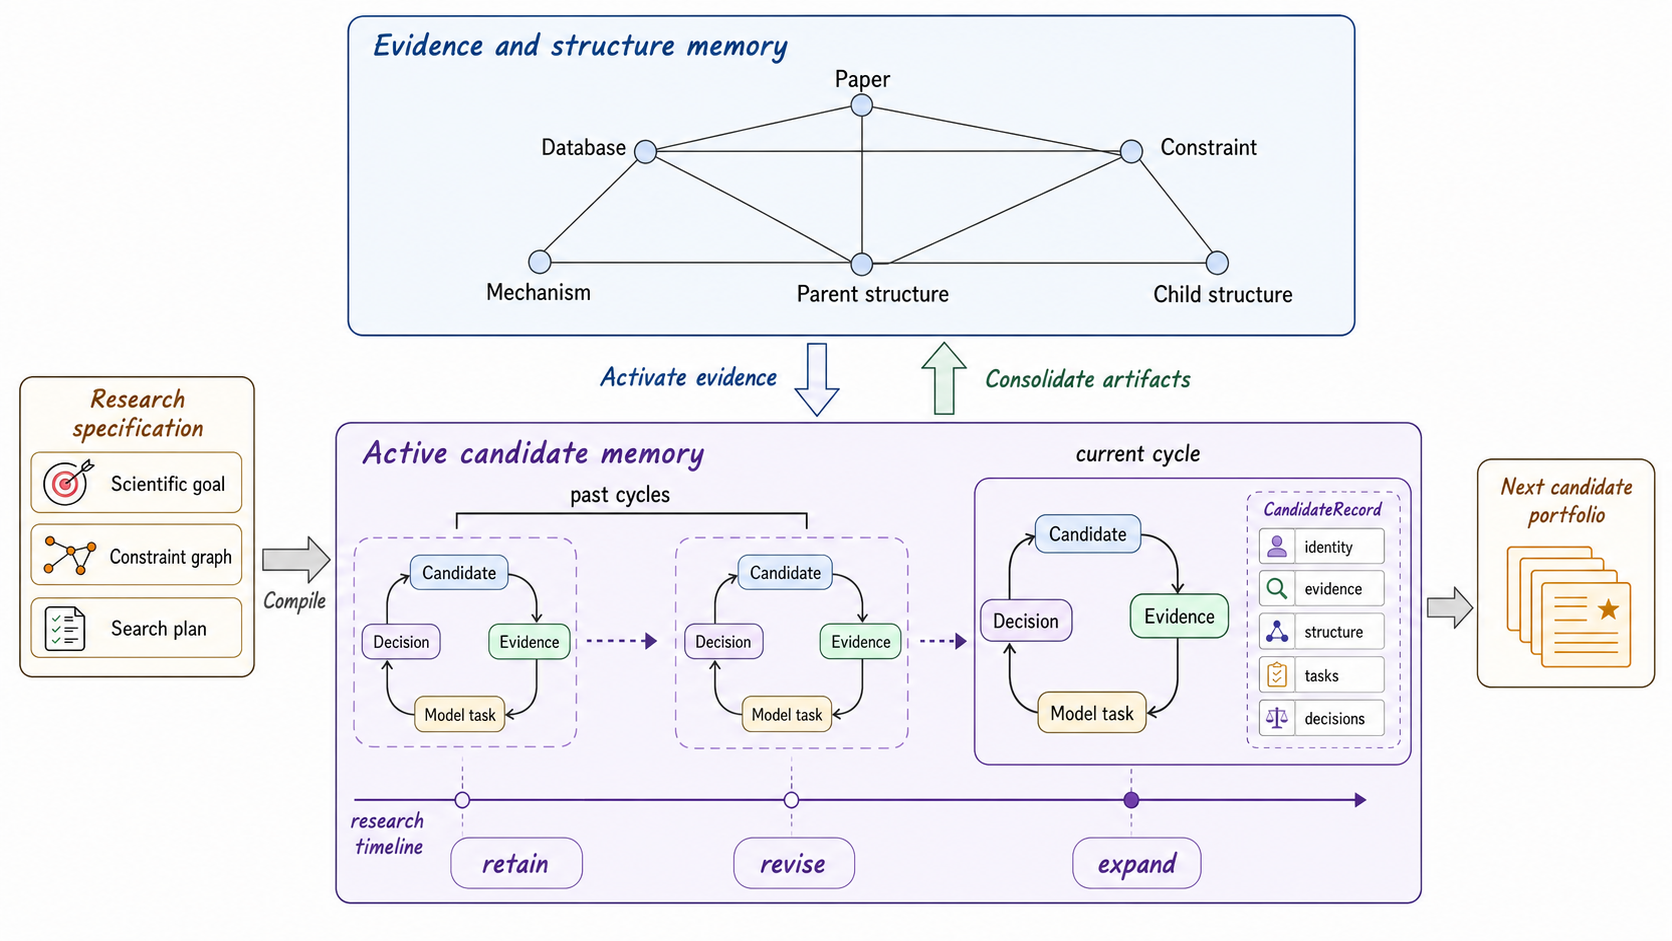
\includegraphics[width=\linewidth]{figures/candidate-artifact-graph-image2-v2.png}
    \caption{\textbf{Candidate-centred scientific memory.}
    Candidate-independent evidence and structures occupy a durable scientific memory, whereas active candidate cycles bind evidence, model tasks, and decisions to a \texttt{CandidateRecord}.  Activation supplies relevant prior artifacts to the current cycle; consolidation writes validated structures and observations back into the shared graph.}
    \label{fig:artifact-graph}
\end{figure}

Figure~\ref{fig:artifact-graph} shows the resulting artifact graph.  An \texttt{EvidenceRecord} stores an observation, its source, retrieval or calculation metadata, and the constraint it can address.  A \texttt{StructureRecord} stores a canonical structure artifact and any transformation that relates it to a parent.  A \texttt{ModelTask} binds an observable to a registered capability and to its input and dependency artifacts.  A \texttt{DecisionRecord} records whether the system retains, revises, or expands a candidate.  These records are individually addressable and are joined through stable candidate identifiers, rather than being embedded only in a final natural-language report.

\subsection{Hermes as the outer research runtime}

\hermes is the outer execution environment of the platform.  A source-controlled \hermes Profile defines the tools visible to the agent, approval policy, time and concurrency limits, and the Skills that specify how a materials campaign is conducted.  The production Profile exposes only bounded materials tools: starting a research run, reading run state, applying an advertised action, reading a verified terminal result, and launching the generic materials-research pipeline.  General terminal, browser, file, and code-execution tools are disabled in this Profile.  This makes the scientific service---rather than an unstructured agent workspace---the authority for candidate state.

The runtime contributes four capabilities.  First, it translates a natural-language goal into a tool-mediated research interaction without requiring the researcher to call individual scientific programs.  Second, it supports long-running runs through explicit state inspection and resumable actions.  Third, it loads distinct materials Profiles for production research, research-only exploration, and controlled evolution.  Fourth, its native memory, Skills, and bounded delegation can be enabled in the evolution Profile to accumulate reusable workflow knowledge while the underlying scientific records remain read-only from that Profile.

This separation is important.  \hermes memory describes how to conduct research; the materials service records what is known about a particular candidate.  The former can improve reusable workflow policy.  The latter preserves structures, evidence, computations, and decisions with scientific provenance.  The two memories interact through reviewed summaries and stable artifact references, but they do not replace one another.

\subsection{The Materials MCP Gateway}

The Materials Model Context Protocol (MCP) Gateway is a narrow interface between the agent runtime and the scientific service.  Its tools use strict input and output schemas and return bounded projections of internal state.  Mutating actions are separated from read-only state and result retrieval.  A run cannot return a terminal result until the authoritative report and its referenced artifacts have been verified by the service.  Requests are idempotently keyed by submission or run identifiers so that an interrupted \hermes interaction can recover an existing campaign instead of silently creating a second one.

The gateway deliberately exposes coarse-grained scientific operations.  For example, the generic materials-research tool initiates the complete evidence and hypothesis workflow; it does not expose a free-form sequence of database queries as independent agent actions.  The underlying service fans out to configured sources, compiles evidence matrices, plans transformations, and constructs model tasks.  This design retains the convenience of natural-language research while keeping identity resolution, scientific verdicts, and structure mutation in deterministic or typed components.

\begin{table}[t]
    \centering
    \caption{\textbf{Division of responsibility between the agent runtime and scientific service.}}
    \label{tab:responsibility}
    \small
    \setlength{\tabcolsep}{5pt}
    \renewcommand{\arraystretch}{1.15}
    \begin{tabularx}{\linewidth}{>{\raggedright\arraybackslash}p{0.18\linewidth}XX}
        \toprule
        \textbf{Layer} & \textbf{Primary responsibility} & \textbf{Persistent output} \\
        \midrule
        \hermes runtime & Dialogue, Profile/Skill policy, agent--tool loop, bounded continuation and workflow evolution & Session state, reusable workflow memory, reviewed Skill updates \\
        Materials MCP Gateway & Schema validation, run admission, action boundary, status and artifact projection & Run identity, action receipts, verified result handles \\
        Materials service & Constraint compilation, evidence federation, structure operations, scientific DAGs and candidate decisions & Candidate, evidence, structure, task and decision records \\
        Scientific backends & Database retrieval, structural checks, learned models, band analysis and first-principles calculations & Source artifacts, model outputs, numerical observations and execution receipts \\
        \bottomrule
    \end{tabularx}
\end{table}

\subsection{End-to-end lifecycle}

A campaign proceeds through five stages.  (1) \matspec compiles the question into typed constraints, permitted modifications, and target observables.  (2) \matevidence retrieves literature and database records, resolves candidate identities, and builds an evidence matrix.  (3) \mattransform converts selected hypotheses into typed structure-operation or condition plans and, where possible, explicit child structures.  (4) \matdag binds candidates to capability-checked model tasks and executes the resulting dependency graph.  (5) \matevolve combines the new artifacts with the current portfolio and produces the next candidate set and validation trajectory.

The lifecycle is not a rigid linear pipeline.  A candidate can return from \matdag to \matevidence when a calculation creates an observation that resolves a previously unknown constraint.  It can return to \mattransform when a result motivates a revised substitution, strain state, or heterostructure.  It can also branch into several descendants while retaining a common parent.  The invariant is that each transition produces a typed artifact and that no observation is detached from the candidate and structure to which it applies.

\subsection{Implementation}

The scientific service is implemented in Python using strict versioned data models.  Structures are stored as content-addressed artifacts, and canonical JSON payloads are hashed to construct deterministic plan identifiers.  The current system includes federated adapters for C2DB, Materials Cloud MC3D, NOMAD, and Materials Project; structure manipulation through an independent soft-chemistry registry; and scientific executors for database electronic structures, structure and energy models, learned Hamiltonians, band analysis, and remote first-principles calculations.  Append-only run directories retain requests, source responses, normalized records, task plans, execution receipts, plots, and reports.  The experiments in Section~\ref{sec:experiments} use these stored artifacts rather than reconstituted examples.
